\documentclass{beamer}\usepackage{graphicx, color}
%% maxwidth is the original width if it is less than linewidth
%% otherwise use linewidth (to make sure the graphics do not exceed the margin)
\makeatletter
\def\maxwidth{ %
  \ifdim\Gin@nat@width>\linewidth
    \linewidth
  \else
    \Gin@nat@width
  \fi
}
\makeatother

\IfFileExists{upquote.sty}{\usepackage{upquote}}{}
\definecolor{fgcolor}{rgb}{0.2, 0.2, 0.2}
\newcommand{\hlnumber}[1]{\textcolor[rgb]{0,0,0}{#1}}%
\newcommand{\hlfunctioncall}[1]{\textcolor[rgb]{0.501960784313725,0,0.329411764705882}{\textbf{#1}}}%
\newcommand{\hlstring}[1]{\textcolor[rgb]{0.6,0.6,1}{#1}}%
\newcommand{\hlkeyword}[1]{\textcolor[rgb]{0,0,0}{\textbf{#1}}}%
\newcommand{\hlargument}[1]{\textcolor[rgb]{0.690196078431373,0.250980392156863,0.0196078431372549}{#1}}%
\newcommand{\hlcomment}[1]{\textcolor[rgb]{0.180392156862745,0.6,0.341176470588235}{#1}}%
\newcommand{\hlroxygencomment}[1]{\textcolor[rgb]{0.43921568627451,0.47843137254902,0.701960784313725}{#1}}%
\newcommand{\hlformalargs}[1]{\textcolor[rgb]{0.690196078431373,0.250980392156863,0.0196078431372549}{#1}}%
\newcommand{\hleqformalargs}[1]{\textcolor[rgb]{0.690196078431373,0.250980392156863,0.0196078431372549}{#1}}%
\newcommand{\hlassignement}[1]{\textcolor[rgb]{0,0,0}{\textbf{#1}}}%
\newcommand{\hlpackage}[1]{\textcolor[rgb]{0.588235294117647,0.709803921568627,0.145098039215686}{#1}}%
\newcommand{\hlslot}[1]{\textit{#1}}%
\newcommand{\hlsymbol}[1]{\textcolor[rgb]{0,0,0}{#1}}%
\newcommand{\hlprompt}[1]{\textcolor[rgb]{0.2,0.2,0.2}{#1}}%

\usepackage{framed}
\makeatletter
\newenvironment{kframe}{%
 \def\at@end@of@kframe{}%
 \ifinner\ifhmode%
  \def\at@end@of@kframe{\end{minipage}}%
  \begin{minipage}{\columnwidth}%
 \fi\fi%
 \def\FrameCommand##1{\hskip\@totalleftmargin \hskip-\fboxsep
 \colorbox{shadecolor}{##1}\hskip-\fboxsep
     % There is no \\@totalrightmargin, so:
     \hskip-\linewidth \hskip-\@totalleftmargin \hskip\columnwidth}%
 \MakeFramed {\advance\hsize-\width
   \@totalleftmargin\z@ \linewidth\hsize
   \@setminipage}}%
 {\par\unskip\endMakeFramed%
 \at@end@of@kframe}
\makeatother

\definecolor{shadecolor}{rgb}{.97, .97, .97}
\definecolor{messagecolor}{rgb}{0, 0, 0}
\definecolor{warningcolor}{rgb}{1, 0, 1}
\definecolor{errorcolor}{rgb}{1, 0, 0}
\newenvironment{knitrout}{}{} % an empty environment to be redefined in TeX

\usepackage{alltt}
\usetheme{Stats}
\setbeamercovered{transparent}
\usepackage{color}
\usepackage{hyperref}
  \hypersetup{
  	colorlinks=true
		linkcolor=black
		}
\usepackage{url}
\usepackage{graphics}
\usepackage{tikz}
\usepackage{booktabs}
\usepackage{multirow}
\usepackage[buttonsize=1em]{animate}





%%%%%%%%%%%%%%%%%%%%%%%%%%%%%%%% Title Slide %%%%%%%%%%%%%%%%%%%%%%%%%%
\title[]{Intro to Social Science Data Analysis \\[1cm] Lecture 9: Overview of Statistical Inference (II)}
\author[]{
    \href{mailto:gandrud@yonsei.ac.kr}{Christopher Gandrud}
}
\date{\today}


\begin{document}

\frame{\titlepage}

\section[Outline]{}
\frame{\tableofcontents}

%%%%%%%%%%% Assignments
\section{Assignments}
\frame{
  \frametitle{General Feedback}
{\Large{Assignment 2 General Feedback}} \\[0.5cm]
  \begin{itemize}
    \item {\bf{Always}} describe your data source.
    \item What do the numbers mean? Remember the units.
    \item What year(s) is the data from?
  \end{itemize}
}

\frame{
	\frametitle{Assignment 3}
  {\Large{Assignment 3}} \\[0.5cm]
  {\bf{Due:}} Friday 16 November \\[0.5cm]
  Have a data set with three variables of the following type:
  \begin{itemize}
    \item 1 numeric variable,
    \item 1 dummy variable,
    \item 1 multinomial variable.
  \end{itemize}
  There should be more than 50 observations per variable \& variable category.
}

\frame{
  \frametitle{Assignment 3}
  {\Large{Find the answers to these questions.}} \\[0.5cm]
Numeric Continuous Variable
  \begin{itemize}
    \item What do you predict the population mean of this variable is? 
    \item Create two groups of this variable based on the dummy variable. Are the population means of these two groups likely to be different?
  \end{itemize}
Dummy Variable
  \begin{itemize}
    \item What are the likely population proportions of the two values of this variable?
  \end{itemize}
Multinomial Variable
  \begin{itemize}
    \item What are the likely population proportions of the values of this variable?
  \end{itemize}
}

%%%%%%%%%%% Recap
\section{Recap}
\frame{
  \frametitle{Intro to Statistical Inference: Quick Quiz (1)}
  Give an example of a population parameter and its corresponding point estimate.
}

\frame{
  \frametitle{Intro to Statistical Inference: Quick Quiz (2)}
  What is the sampling distribution of the sampling mean? \\[0.5cm]
  In general, what is the sampling distribution of the sampling mean centered on?
}

\frame{
  \frametitle{Intro to Statistical Inference: Quick Quiz (3)}
  What do we use to find the standard error of a point estimate? \\[0.5cm]
  What do we use the standard error for?
}

\frame{
  \frametitle{Intro to Statistical Inference: Quick Quiz (4)}
  What is a confidence interval? \\[0.5cm]
  Why is it more useful to show the confidence interval than just the standard error?
}

\frame{
  \frametitle{Today}
{\Large{Last class we largely looked at how to draw inferences about a population {\bf{mean}} from a sample {\bf{mean}}.  }} \\[0.5cm]
  Today we will expand our inferential tools by learning about:
  \begin{itemize}
    \item Hypothesis testing including $\mathrm{Z}$ scores, $t$ distributions, \& p-values,
    \item Comparing 2 population means,
  \end{itemize}
  Next class:
  \begin{itemize}
    \item Making inferences with population proportions,
    \item Inferential statistics with categorical variables.
  \end{itemize}

}

%%%%%%%%%%% Hypothesis testing
\section{Hypothesis Testing: Overview}
\begin{frame}[fragile]
  \frametitle{Hypothesis Testing Setup}
  {\large{Imagine that we have a sample of 200 Cherry Blossom Run Finishing times from the 2009 race. \\[0.25cm] (This example is largely from Diaz et al. 2011. See last week's lecture for more details) \\[0.5cm]



  The mean finishing time in the sample is 93.9 minutes with a standard deviation of 15.6}}
\end{frame}

\frame{
  \frametitle{Question}
{\Large{The mean finishing time in 2006 was 93.29. \\[0.5cm]
  Is there strong evidence that on average the 2009 runners are faster/slower than the 2006 runners?}}
}

\frame{
  \frametitle{The language of hypothesis testing.}
  {\large{We can think that there are two {\bf{competing}} possibilities: \\[0.5cm]
  \begin{itemize}
    \item $H_{0}$: There is {\emph{no difference}} in the average finishing times between the 2006 and 2009 runners ({\bf{the null hypothesis}}).
    \item $H_{a}$: The average finishing time in 2006 {\emph{is different}} from the average finishing time in 2009 ({\bf{the alternative hypothesis}}). 
  \end{itemize}
  }}
}

\frame{
  \frametitle{The language of hypothesis testing}
{\large{In other words, if the population mean for the 2009 is called $\mu_{09}$: \\[0.5cm]
  \begin{itemize}
    \item $H_{0}: \mu_{09} = 93.29$
    \item $H_{A}: \mu_{09} \neq 93.29$
  \end{itemize} \\[0.5cm]
  93.29 is called the {\bf{null value}}, as it is the value of the parameter {\bf{if}} the null hypothesis is true.
}}
}

\frame{
  \frametitle{The language of hypothesis testing}
{\large{The null hypothesis is the {\bf{skeptical possibility}}. \\[0.5cm]
  If we do not find evidence against the null hypothesis we say that we: {\emph{fail to reject the null hypothesis.}} \\[0.5cm]
  If we do find evidence against the null hypothesis we say that we: {\emph{found evidence for the alternative hypothesis.}}
  }}
}

\frame{
  \frametitle{Evidence}
{\Large{What kind of evidence can we use to either reject or fail to reject the null hypothesis?}}
}

\frame{
  \frametitle{Evidence}
  \begin{center}
{\Large{Confidence intervals!}}
  \end{center}
}

\begin{frame}[fragile]
  \frametitle{95\% Confidence Interval for 2009 Mean Finishing Times ($n = 200$)}
\begin{knitrout}
\definecolor{shadecolor}{rgb}{0.969, 0.969, 0.969}\color{fgcolor}

{\centering 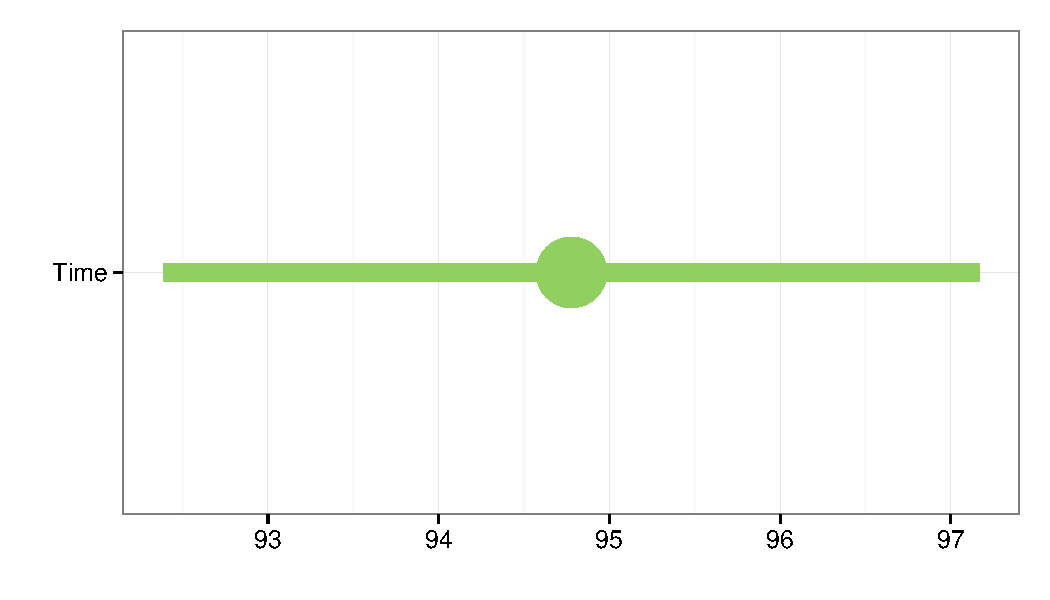
\includegraphics[width=\maxwidth]{figure/TimeCI} 

}


\end{knitrout}

\end{frame}

\begin{frame}[fragile]
  \frametitle{95\% Confidence Interval for 2009 Mean Finishing Times ($n = 200$) Compared to the Null Hypothesis}
\begin{knitrout}
\definecolor{shadecolor}{rgb}{0.969, 0.969, 0.969}\color{fgcolor}

{\centering 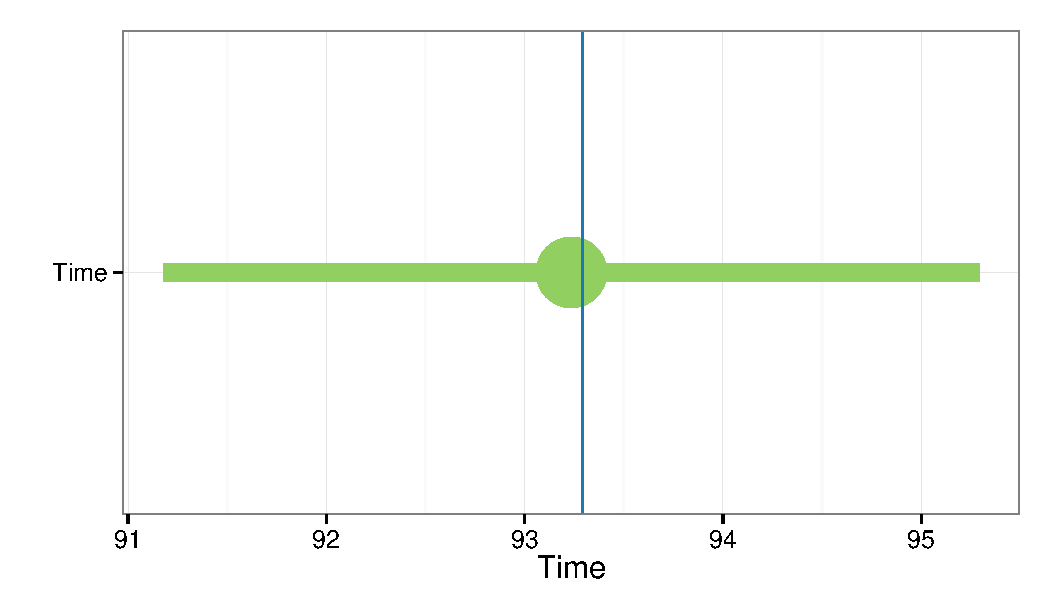
\includegraphics[width=\maxwidth]{figure/TimeCINull} 

}


\end{knitrout}

\end{frame}

\frame{
  \frametitle{Fail to Reject}
{\Large{The 2006 population mean is inside of the 95\% confidence interval of the 2009 sample estimate. \\[0.5cm]
  Therefore, we {\emph{fail to reject}} the null hypothesis that the 2009 Cherry Blossom Run mean finishing time is different from the 2006 mean finishing time.}}
}

\frame{
  \frametitle{Be Careful}
{\Large{Be Careful: Hypothesis testing is far from perfect. \\[0.5cm]  
  }}
{\small{
  \begin{table}
    \begin{tabular}{c c | c c}
    & & \multicolumn{2}{c}{{\bf{Test Conclusion}}} \\[0.25cm]
    \hline
    & & Do Not Reject $H_{0}$ & Reject in favour of $H_{A}$ \\[0.25cm]
    \hline
    \multirow{2}{*}{{\bf{Real World}}} & $H_{0}$ True & okay & Type 1 Error \\[0.25cm]
    & $H_{A}$ True & Type II Error & okay \\
    \hline
    \end{tabular}

  \end{table}
  (Diaz et al. 2001, 160)
}}
}

%%%%%%%%%%%% Z Scores & t distributions
\section{$\mathrm{Z}$ Scores and $t$ Distributions}
\frame{
  \frametitle{Quantifying Error Probabilities}
  We previously used a 95\% confidence interval to test the Null Hypothesis. \\[0.5cm]
  This means that 5\% of the time we will {\bf{incorrectly}} reject $H_{0}$ due to {\bf{sampling variation}}. \\[0.25cm]
  2.5\% of the time the confidence interval will be {\bf{too high}}. \\
  2.5\% of the time the confidence interval will be {\bf{too low}}.\\[0.5cm]
  This is also called the 95\% {\bf{significance level}} or sometimes $\alpha = 0.05$.
}

\begin{frame}[fragile]
  \frametitle{Remember: Confidence Interval Simulation}
\begin{knitrout}
\definecolor{shadecolor}{rgb}{0.969, 0.969, 0.969}\color{fgcolor}

{\centering \animategraphics[,controls,loop]{1}{figure/CIRememberAnimation}{1}{50}

}


\end{knitrout}

\end{frame}

\frame{
  \frametitle{Higher Confidence}
  {\Large{If we use a {\bf{higher significance level}} we will be more confident that we correctly rejected or failed to reject the null hypothesis. \\[0.5cm]
  For example, at the {\bf{99\% significance level}} we will incorrectly reject the $H_{0}$ 1\% of the time.}}
}

\frame{
  \frametitle{99\% Confidence Interval}
{\LARGE{The 99\% Confidence Interval of the Mean: \\[0.5cm]
  \[
    CI_{99\%} = \bar{x} \pm 2.58 * SE_{\bar{x}}
  \]
  }}
}

\begin{frame}[fragile]
  \frametitle{Comparing Confidence Intervals}



\begin{knitrout}
\definecolor{shadecolor}{rgb}{0.969, 0.969, 0.969}\color{fgcolor}

{\centering 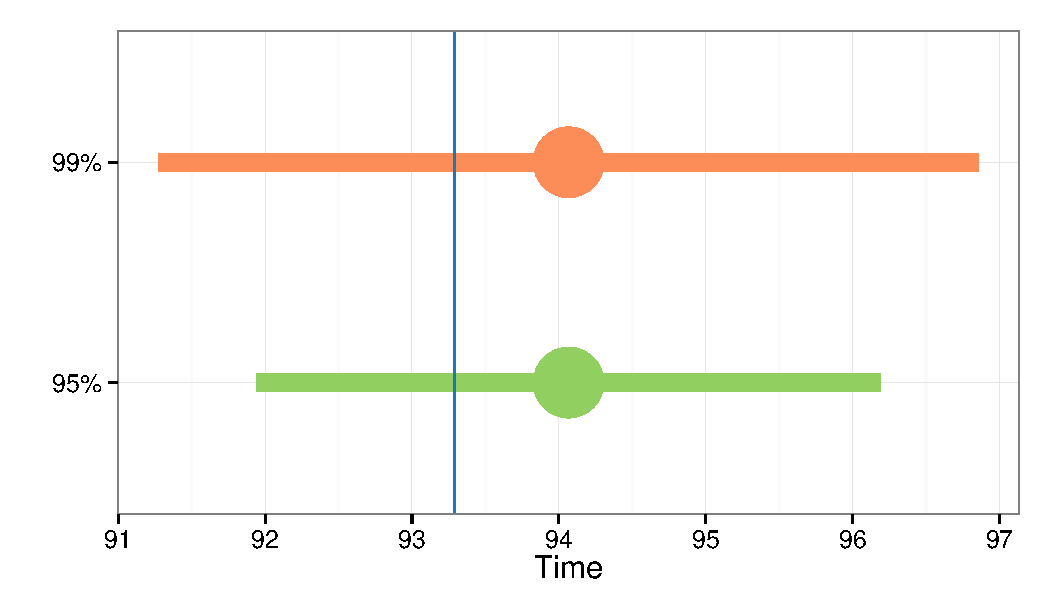
\includegraphics[width=\maxwidth]{figure/PlotCICompare} 

}


\end{knitrout}

\end{frame}

\frame{
  \frametitle{Confidence Intervals and \mathrm{Z} Scores}
  \begin{center}
{\Large{Where does the 2.58 come from? \\[0.5cm]
  Where does the 1.96 come from (for 95\% confidence intervals)? }}
  \end{center}
}

\frame{
  \frametitle{Confidence Intervals and \mathrm{Z} Scores}
{\large{They are the $\mathrm{Z}$ score for the confidence level. \\[0.5cm]
  $\mathrm{Z}$ scores are the number of standard deviations above or below the mean that an observation falls.\\[0.5cm]
  Because of the Central Limit Theorem, if 
  \begin{itemize}
    \item<1-> the sample observations are {\bf{independent}},
    \item<1-> the sample size is {\bf{large}} (about $n \geq 50$),
    \item<1-> the distribution is {\bf{not extremely skewed}}.
  \end{itemize}
  then we can assume that\ldots
  }}
}

\begin{frame}
  \frametitle{$\mathrm{Z}$ Scores and Confidence Intervals}
  \begin{center}
    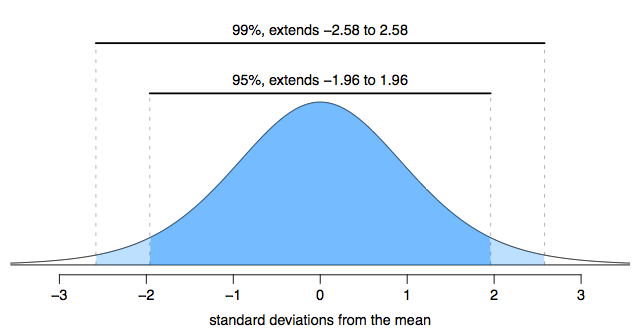
\includegraphics[scale=0.45]{figure/ZScore.png} \\
    Source: Diaz et al. (2011, 154)
  \end{center}
\end{frame}

\frame{
  \frametitle{What if the Central Limit Theorem's Assumptions Aren't Met?}
{\Large{What if the Central Limit Theorem's Assumptions Aren't Met?}} \\[0.5cm]
  \begin{itemize}
    \item Dependent data: See Sainani (2010): \url{http://www.stanford.edu/~kcobb/hrp259/correlateddata.pdf}. 
    \item The larger the sample, the more lenient you can be about skewness.
    \item If you have a smaller sample size and it is skewed, you can use a version of the Wilcox test (in R \texttt{Wilcox.test}) for hypothesis testing. See Crawley (2005, Ch. 5)
    \item If you have a small sample (about $n < 50$) that is not highly skewed, you can use the $t$ distribution to calculate confidence intervals. In R use \texttt{t.test}. See Diaz et al. (2011, Ch. 6).
  \end{itemize}
}

\begin{frame}
  \frametitle{The $t$ distribution with various Degrees of Freedom}
  \begin{center}
    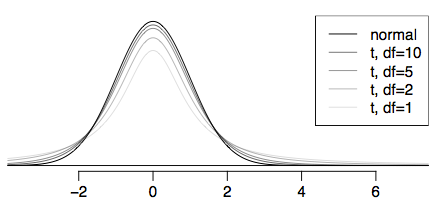
\includegraphics[scale=0.5]{figure/tDist.png} \\
    df = Degrees of Freedom ($n - 1$)\\[0.25cm]
    {\tiny{Source: Diaz et al. (2011, 244)}}
  \end{center}
\end{frame}

%%%%%%%%%%%% p-values
\section{p-values}
\frame{
  \frametitle{p-values}
  {\Large{Some researchers like to quantify the strength of the evidence against the Null Hypothesis with a tool called the {\bf{p-value}}.}}
}

\begin{frame}[fragile]
  \frametitle{What is the p-value}
{\LARGE{p-value}} \\[0.5cm]
  The probability of seeing data at least as favourable to the alternative hypothesis as our current data, {\emph{if the null hypothesis is true}}. \\[0.5cm]
  In our previous {\bf{example}}, we would want to know the probability of seeing a mean of at least 94.5 if the true population mean is actually 93.29 (the population mean for 2006).
\end{frame}

\begin{frame}[fragile]
  \frametitle{Visualizing the p-value}
  \begin{center}
    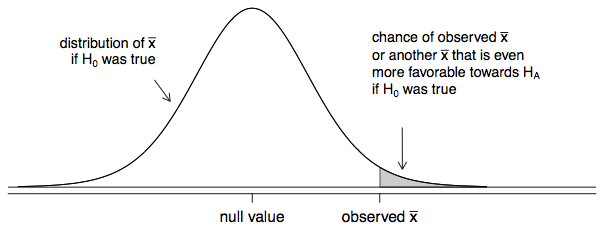
\includegraphics[scale=0.5]{figure/AbstractP.png}
  \end{center}
\end{frame}

\begin{frame}[fragile]
  \frametitle{Example}
{\LARGE{Example}} \\[0.5cm]
  In our previous {\bf{example}}, we would want to know the probability of seeing a mean of at least 94.5 if the true population mean is actually 93.29 (the population mean for 2006). \\[0.5cm]
\end{frame}

\begin{frame}[fragile,plain]
{\LARGE{1st: Test Statistic}} \\[0.5cm]
  We first calculated the $\mathrm{Z}$ score {\bf{test statistic}} of the sample mean $\bar{x} = 94.5$
\[
  \mathrm{Z} = \frac{\bar{x} - \mathrm{null\:value}}{SE_{\bar{x}}}
\]\\[0.25cm]
In R:
\begin{knitrout}
\definecolor{shadecolor}{rgb}{0.969, 0.969, 0.969}\color{fgcolor}\begin{kframe}
\begin{alltt}
\hlcomment{# Load library}
\hlfunctioncall{library}(plotrix)

\hlcomment{# Find Z score }
Z <- (\hlfunctioncall{mean}(Run10Samp$time) - 93.29)/
      \hlfunctioncall{std.error}(Run10Samp$time)

Z
\end{alltt}
\begin{verbatim}
## [1] 0.5559
\end{verbatim}
\end{kframe}
\end{knitrout}

\end{frame}

\begin{frame}
  \frametitle{$\mathrm{Z}$ Scores and Confidence Intervals}
  \begin{center}
    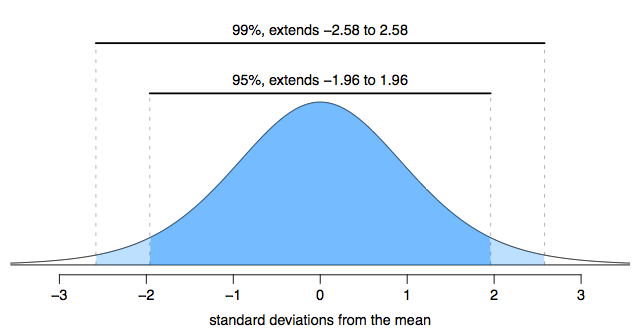
\includegraphics[scale=0.45]{figure/ZScore.png} \\
    Source: Diaz et al. (2011, 154)
  \end{center}
\end{frame}

\begin{frame}[fragile]
{\LARGE{2nd: Find p-values}}
  To find the p-value for the 0.6 use \texttt{pnorm}.
\begin{knitrout}
\definecolor{shadecolor}{rgb}{0.969, 0.969, 0.969}\color{fgcolor}\begin{kframe}
\begin{alltt}
P1 <- 1 - \hlfunctioncall{pnorm}(Z)
P1
\end{alltt}
\begin{verbatim}
## [1] 0.2891
\end{verbatim}
\end{kframe}
\end{knitrout}

So, if the null hypothesis was true we would have a 0.2891 probability of observing a mean of at least 0.6 larger than the 2006 mean. \\[0.25cm]
This is bigger than the 0.05 significance level. So, we fail to reject the null hypothesis that $\mu_{{x}_{09}} > \mu_{{x}_{06}}$.
\end{frame}

\begin{frame}[fragile]
  \frametitle{Um\ldots}
  But we were interested in the null hypothesis $\mu_{{x}_{09}} = \mu_{{x}_{06}}$, not $\mu_{{x}_{09}} > \mu_{{x}_{06}}$. \\[0.5cm]
  So far we have only looked one tail of the distribution. To examine both tails simply {\bf{multiply the one-tail p-value by 2}}.
\begin{knitrout}
\definecolor{shadecolor}{rgb}{0.969, 0.969, 0.969}\color{fgcolor}\begin{kframe}
\begin{alltt}
P2 <- 2 * (1 - \hlfunctioncall{pnorm}(Z))

P2
\end{alltt}
\begin{verbatim}
## [1] 0.5782
\end{verbatim}
\end{kframe}
\end{knitrout}

We fail to reject the null hypothesis that $\mu_{{x}_{09}} = \mu_{{x}_{06}}$. \\[0.25cm]
In other words, we have evidence that there is no difference in the mean finishing times from the 2006 and 2009 Cherry Blossom Run.

\end{frame}

%%%%%%%%%%% Comparing 2 Means
\section{Comparing Two (Independent) Means}
\frame{
  \frametitle{Comparing Means}
  \begin{center}
{\LARGE{Comparing Means}}
  \end{center}
}

\frame{
  \frametitle{Question}
  \begin{center}
  Are men's finishing times different than women's finishing time in the 2009 Cherry Blossom Run?
  \end{center}
}

\begin{frame}[fragile]
  \frametitle{Summary Descriptives}


  
  \begin{table}
  \caption{Descriptive Statistics of the Sample}
  \begin{tabular}{c | c c c}
  & $\bar{x}$ & $s$ & $n$ \\
  \hline\hline
  Female & 98.9 & 14.2 & 105 \\
  Male & 88.3 & 15.3 & 95 \\
  \hline
  
  \end{tabular}
  \end{table}
\end{frame}

\begin{frame}[fragile,plain]
\begin{knitrout}
\definecolor{shadecolor}{rgb}{0.969, 0.969, 0.969}\color{fgcolor}\begin{kframe}
\begin{alltt}
\hlcomment{# Compare densities of Men/Women Times}
\hlfunctioncall{ggplot}(Run10Samp, \hlfunctioncall{aes}(y = time, 
                      x = gender, color = gender)) +
        \hlfunctioncall{geom_boxplot}() +
        \hlfunctioncall{theme_bw}()
\end{alltt}
\end{kframe}

{\centering 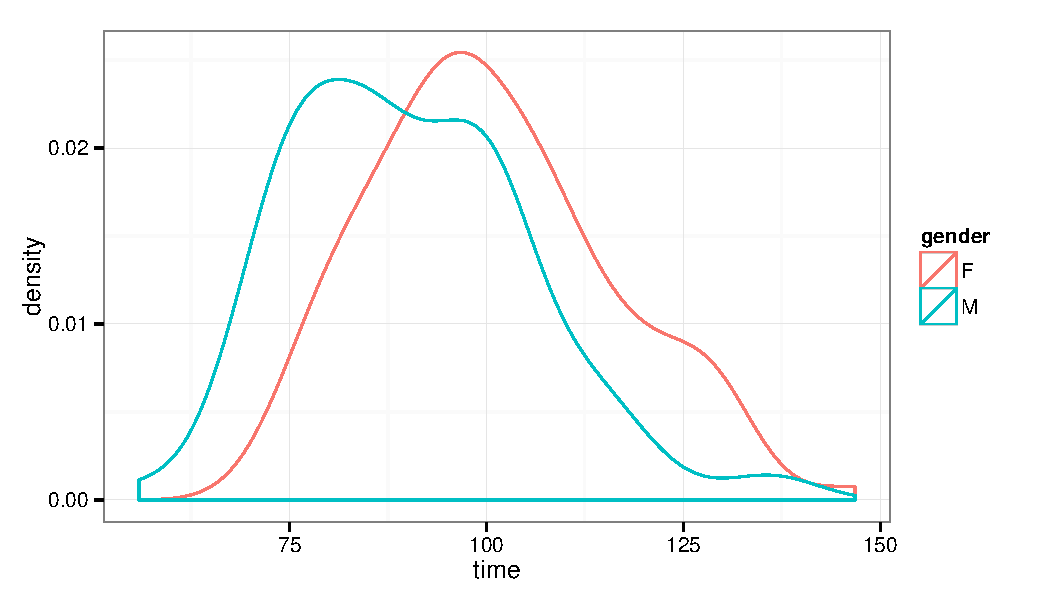
\includegraphics[width=\maxwidth]{figure/GenderDist} 

}


\end{knitrout}

\end{frame}

\frame{
  \frametitle{Comparing Two Means: Hypothesis Testing}
  {\Large{Null Hypothesis: 
  \begin{center}
    $\mu_{m} = \mu_{w}$ \\[0.25cm]
  \end{center}
  Alternative Hypothesis: 
  \begin{center}
    $\mu_{m} \neq \mu_{w}$ \\[0.5cm]
  \end{center}
  An equivalent way to write this null hypothesis is: 
  \begin{center}
    $\mu_{m} - \mu_{w} = 0$
  \end{center}
  }}
}

\begin{frame}[fragile]
  \frametitle{Our Sample}
  The {\bf{difference in mean}} times between Men and Women is:
  \begin{center}
    $\mu_{m} - \mu_{w}$ \\[0.25cm]
    88.3 - 98.9 = -10.6
  \end{center}
\end{frame}

\begin{frame}[fragile]
  \frametitle{Standard Error of the Difference of Two Means}
{\Large{Standard Error of the Difference of Two Means:}}
\[
  SE_{\bar{x}_{m} - \bar{x}_{w}} = \frac{\sigma_{m}}{\sqrt{n_{m}}} + \frac{\sigma_{w}}{\sqrt{n_{w}}}
\] \\[0.5cm]
\end{frame}

\begin{frame}[fragile]
  \frametitle{Approximate the Standard Error.}
  Because in our sample each gender has {\bf{more than 50 observations}} that are {\bf{independent}}, and the is {\bf{normally distributed}} we can use the {\bf{sample standard deviations}} to approximate the standard error of the difference of two means:
\[
  SE_{\bar{x}_{m} - \bar{x}_{w}} = \frac{\sigma_{m}}{\sqrt{n_{m}}} + \frac{\sigma_{w}}{\sqrt{n_{w}}} \approx \frac{s_{m}}{\sqrt{n_{m}}} + \frac{s_{w}}{\sqrt{n_{w}}} = \frac{15.3}{\sqrt{95}}} + \frac{14.2}{\sqrt{105}}
\]\\[0.5cm]
\[
SE_{\bar{x}_{m} - \bar{x}_{w}} = 2.9565
\]
\end{frame}

\begin{frame}[fragile]
  \frametitle{The R Code}
{\Large{Here is the R Code for Everything We Need (1)}}
\begin{knitrout}
\definecolor{shadecolor}{rgb}{0.969, 0.969, 0.969}\color{fgcolor}\begin{kframe}
\begin{alltt}
\hlcomment{# Subset Samples}
MenSubset <- \hlfunctioncall{subset}(Run10Samp$time, 
                       Run10Samp$gender == \hlstring{"M"})
WomenSubset <- \hlfunctioncall{subset}(Run10Samp$time, 
                       Run10Samp$gender == \hlstring{"F"})

\hlcomment{# Means}
MeanMen <- \hlfunctioncall{mean}(MenSubset)
MeanWomen <- \hlfunctioncall{mean}(WomenSubset)

\hlcomment{# Mean difference}
MeanDiff <- MeanMen - MeanWomen
\end{alltt}
\end{kframe}
\end{knitrout}

\end{frame}

\begin{frame}[fragile]
  \frametitle{The R Code}
{\Large{Here is the R Code for Everything We Need (2)}}
\begin{knitrout}
\definecolor{shadecolor}{rgb}{0.969, 0.969, 0.969}\color{fgcolor}\begin{kframe}
\begin{alltt}
\hlcomment{# Standard Errors}
SEMen <- \hlfunctioncall{std.error}(MenSubset)
SEWomen <- \hlfunctioncall{std.error}(WomenSubset)

\hlcomment{# Standard error of the difference of two means}
SEDiff <- SEMen + SEWomen
\end{alltt}
\end{kframe}
\end{knitrout}

\end{frame}

\begin{frame}[fragile]
  \frametitle{Hypothesis Testing}
{\Large{Now that we have the difference in means, the standard error of the difference in means, and the sample sizes we can statistically examine whether or not the mean finishing times are different for men and women.}}
\end{frame}

\begin{frame}[fragile]
  \frametitle{Confidence Intervals}
{\Large{Let's find the 95\% Confidence interval of the Difference of the Two Means}}
\begin{knitrout}
\definecolor{shadecolor}{rgb}{0.969, 0.969, 0.969}\color{fgcolor}\begin{kframe}
\begin{alltt}
\hlcomment{# Lower bound of the confidence interval}
Lower <- MeanDiff - 1.96 * SEDiff

\hlcomment{# Upper bound of the confidence interval}
Upper <- MeanDiff + 1.96 * SEDiff

Lower
\end{alltt}
\begin{verbatim}
## [1] -16.4
\end{verbatim}
\begin{alltt}
Upper
\end{alltt}
\begin{verbatim}
## [1] -4.81
\end{verbatim}
\end{kframe}
\end{knitrout}

\end{frame}

\begin{frame}[fragile]
  \frametitle{Better}
\begin{knitrout}
\definecolor{shadecolor}{rgb}{0.969, 0.969, 0.969}\color{fgcolor}

{\centering 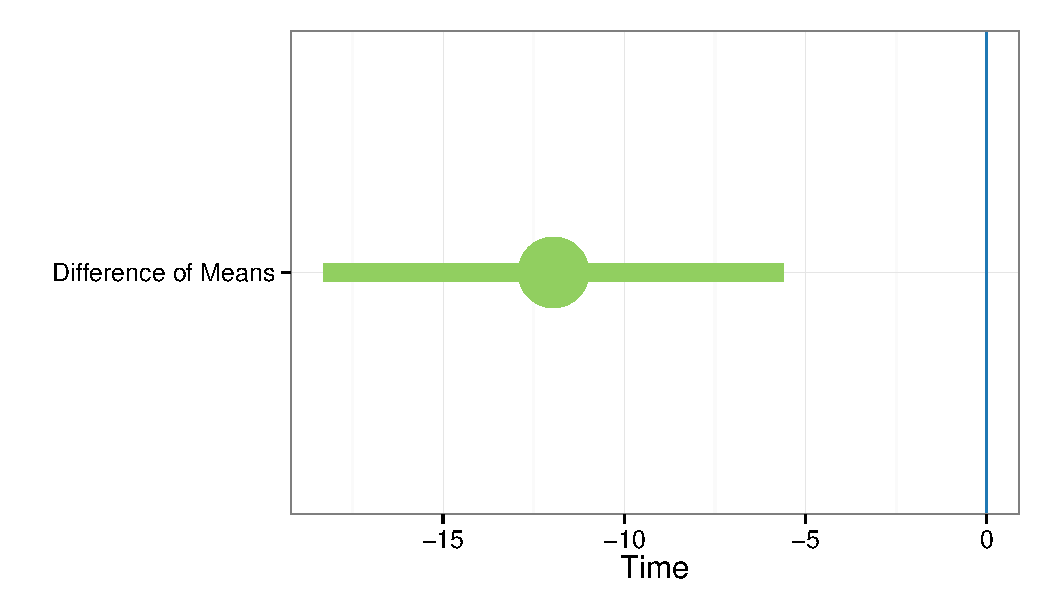
\includegraphics[width=\maxwidth]{figure/PlotCIDiffMeans} 

}


\end{knitrout}

\end{frame}

\frame{
  \frametitle{Substantive Interpretation}
{\large{So, we can reject the null hypothesis that $\mu_{m} - \mu_{w} = 0$ \\[0.5cm]
I.e. we have evidence that women's and men's finishing times in the 2009 Cherry Blossom Race were different.}}
}


\begin{frame}[allowframebreaks]
  \frametitle{References}
  Crawley, Michael J. 2005. Statistics: An Introduction Using R. Chichester: John Wiley & Sons. Ltd. \\[0.25cm]
  Diaz, David M., Christopher D. Barr, and Mine \c{C}etinkaya-Rundel. 2011. OpenIntro Statistics. 1st ed. \url{http://www.openintro.org/stat/downloads.php}. \\[0.25cm] 
\end{frame}


\end{document}
